\documentclass[]{article}
\usepackage{float, graphics, graphicx}

\title{Lux: A Distributed Multi-GPU System for Fast Graph Processing}
\author{1665528-Emiliano Luci, 1665803-Federico Trombetti}

\begin{document}

\maketitle

\section{Introduction}
\subsection{Description of the problem}
Graph application have a high ratio of random memory accesses / actual computation done and are often embarrassingly parallel. It thus makes sense to leverage an architecture with a very high memory bandwidth and a high number of computational units. Fortunately, GPUs clusters are a thing that exists. 

\begin{figure}[H]

	\centering
	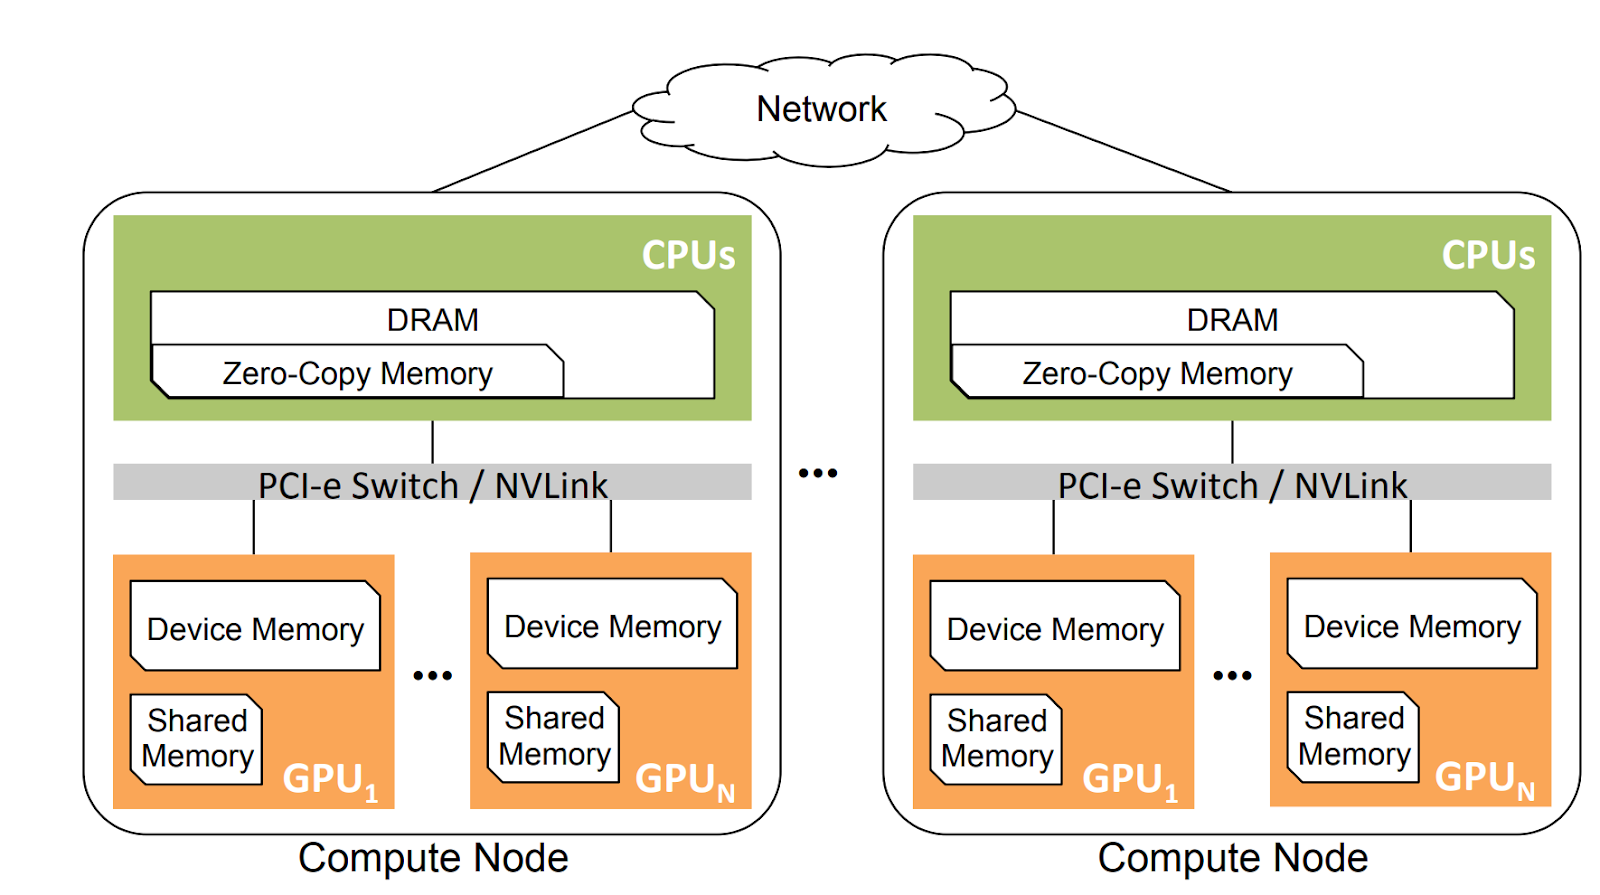
\includegraphics[width=0.7\linewidth]{gpu_cluster.png}
	\caption{The structure of a GPUs cluster}
	\label{fig:gpu_cluster}
\end{figure}

As we can see in Fig.\ref{fig:gpu_cluster} GPUs clusters have a very heterogeneous structure. In order to exploit the full potential of such a system one needs to build a framework that
\begin{itemize}
	\item Distributes the graph efficiently amongst devices and within each device amongst the memories hierarchy.
	\item Find the best way to maximize locality in the memory access of the hierarchy.
	\item Minimize frequent uncoalesced updates to the graph ( i.e. minimize the need for inter-node and inter-device communication).
\end{itemize}

\subsection{Current approaches}
Many framework exists for graph processing. We will quickly go over them and where they present room for improvement:
\begin{itemize}
	\item \textbf{Distributed CPU-based systems}: CPUs are usually more limited in number of cores, large clusters imply greater message passing, access to DRAM is slow and not optimized for coalesced requests.
	\item \textbf{Single-Node CPU-based systems}: While this approach eliminates the need for inter-node communication it suffers from the same problems of untapped parallelization and memory bottleneck.
	\item \textbf{GPU-based systems}: the currently existing frameworks focus on single machine - multi GPUs systems and present do not fully exploit the internal optimizations done by GPUs nor present a good approach to move data between memory hierarchies.
\end{itemize}
 
 \section{Contribution of the paper}
 We will now go through the framework structure and how the authors approached the problems presented.
 \subsection{The computation model}
 
 
 
 
\section{Critique}
We will now present some possible critiques to the paper. The first one is how, much like other frameworks, Lux forces the user to cast their algorithm into a rigidly fixed interface. While this may fit many problems from other existing examples of such an approach we imagine that there will be algorithms that must take an awkward form to fit into Lux's program interface.

\end{document}
